\graphicspath{{members/ssr/figures/}}

\subsection{Greenhouse}\label{subsec:greenhouse}

A greenhouse is a special building for the lone purpose of growing plans under optimal
conditions.
It‘s build of (semi)transparent walls and a roof - depending on the specific
needs of the crops and the location.
Environmental controls govern the atmosphere - ideally - for optimal growing conditions.
The controls typically regulate temperature, humidity, lighting, irrigation and the
nutrition provided through the soil etc.\\

\begin{figure}[H]
    \centering
    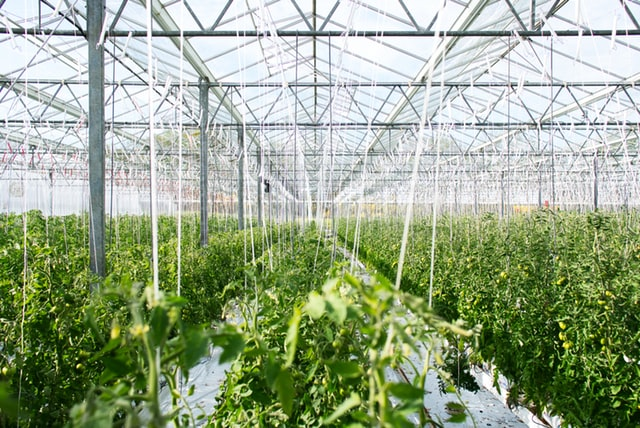
\includegraphics[width=0.8\textwidth]{user-view/greeenhouse_erwan_hesry_unsplash.jpg}
    \caption{Inside a greenhouse}
\end{figure}

Only crops with similar or same optimal growing conditions are grown within each greenhouse
since different crops have difference optimal growing conditions but typically only one crop
variety is grown within each greenhouse.\\

While the greenhouse system won't be introduced here further - since it's not the focus
of this project - it's nonetheless worthwhile to get a high-level picture of the
greenhouse as a controlled environment.
Figure \ref{fig:scheme:greenhouse} provides a schematic overview which shows the external
disturbance variables which impair the greenhouse regulation and the controlled variables.

\begin{figure}[H]
    \centering
    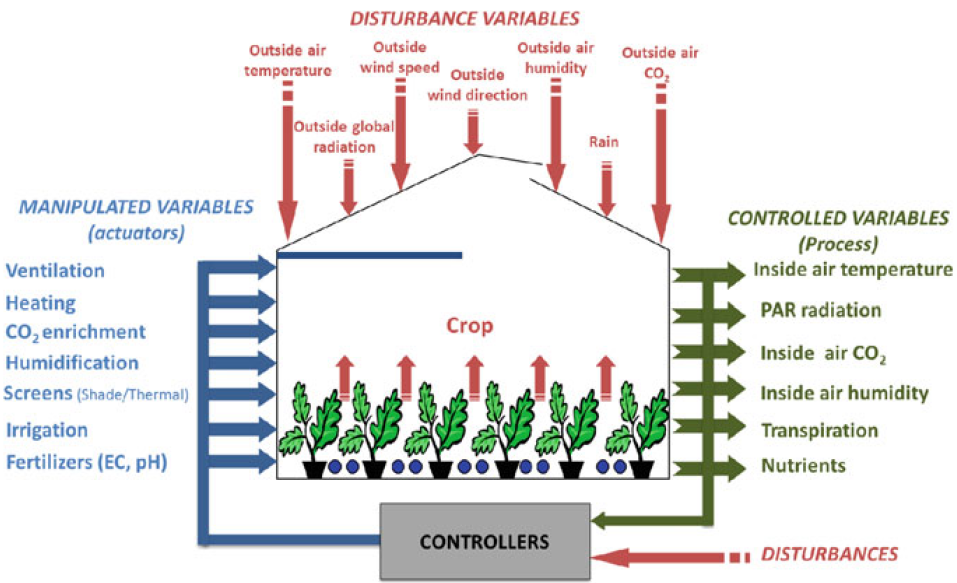
\includegraphics[width=1.0\textwidth]{user-view/climate-control-scheme.png}
    \caption{Greenhouse as a controlled environment with controlled variables and disturbance factors \cite{rod:greenhouse}}
    \label{fig:scheme:greenhouse}
\end{figure}

\subsubsection*{Greenhouse layout and support structures}

The greenhouse's layout is arranged in ways to optimally make use of the available space by densely
arranging the crops.
Since most greenhouses are used for commercial purposes and in this setting the yield per ground
unit is pivotal the goal is to maximize the yield of each plant.\\

In order to archive this goal, the crops are closely planted next to each other in rows
or lanes with just enough room in between to be accessed by workers (figure \ref{fig:lane1}, \ref{fig:lane2}).

\begin{figure}[H]
    \centering
    \begin{minipage}[b]{0.47\textwidth}
        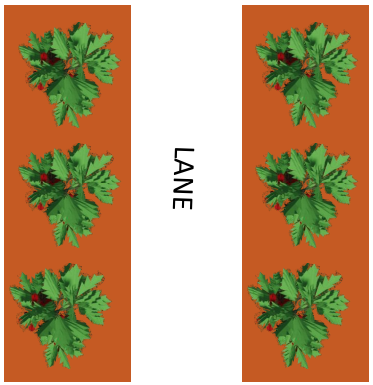
\includegraphics[width=\textwidth]{user-view/lanes.png}
        \caption{Crops arranged in lanes}
        \label{fig:lane1}
    \end{minipage}
    \hfill
    \begin{minipage}[b]{0.49\textwidth}
        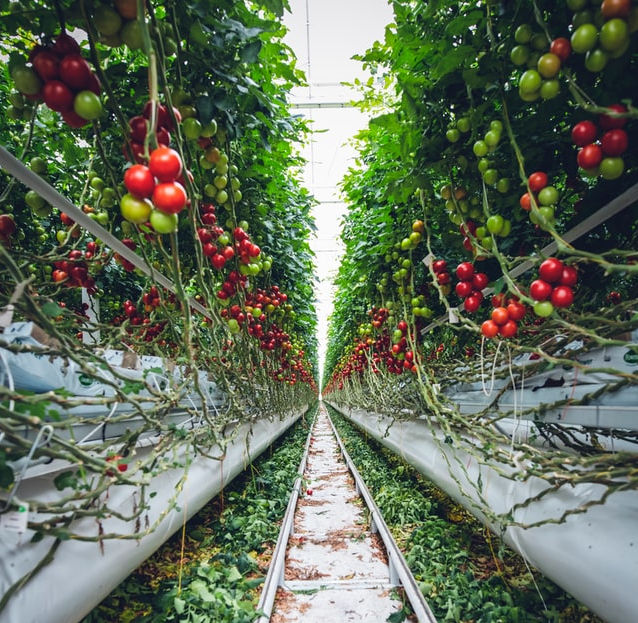
\includegraphics[width=\textwidth]{user-view/plant1_markus_spiske_unsplash.jpg}
        \caption{Walkable lanes}
        \label{fig:lane2}
    \end{minipage}
\end{figure}

Each single plant is supported by a stake which is an effective support structure to ensure
the stability of the tomato plant.
The material and type of the support structure can vary from cage-like structures
to a more common single vertical stake made from any available straight material (figure \ref{fig:stake})
which keeps the plant straight.

\begin{figure}[H]
    \centering
    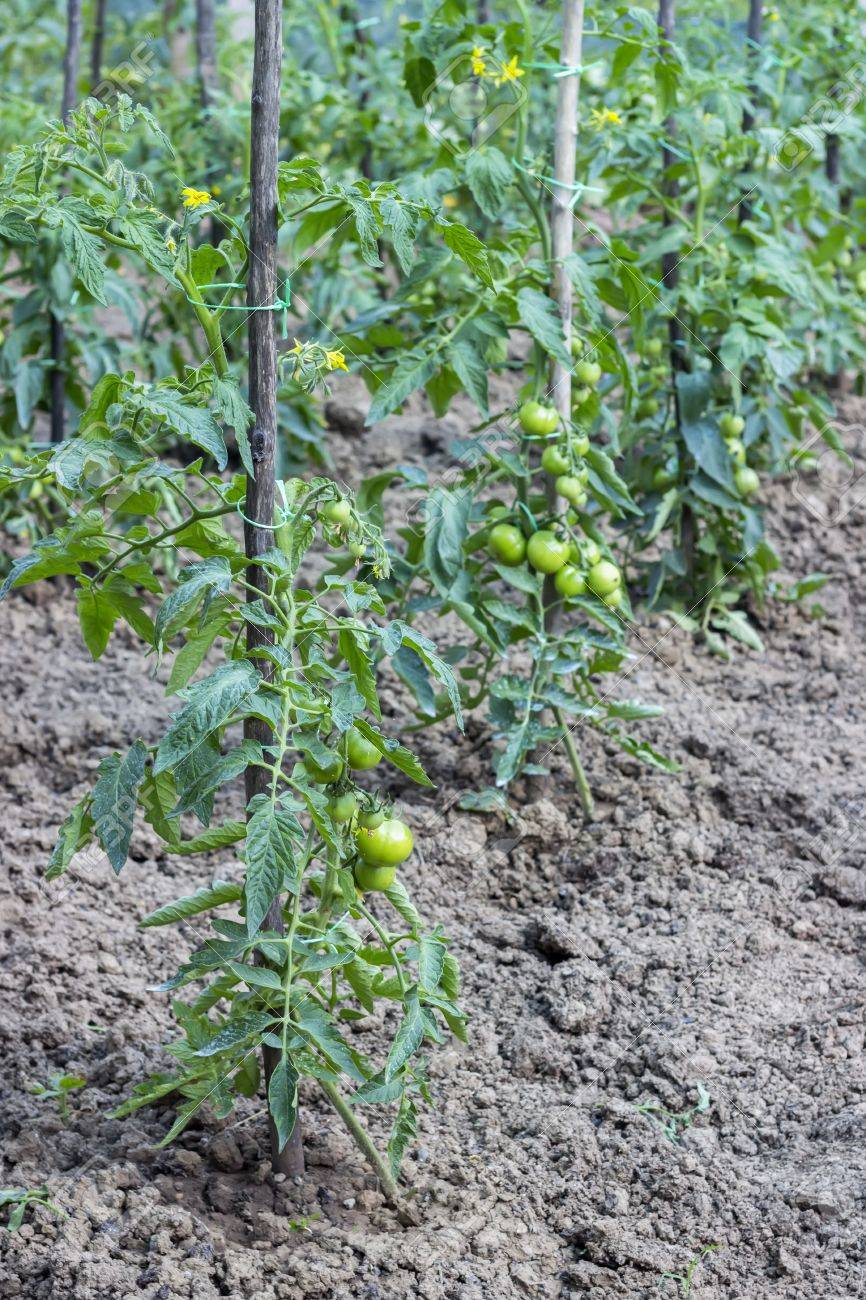
\includegraphics[width=0.3\textwidth]{user-view/tomato_stake.jpg}
    \caption{Plants supported by stakes}
    \label{fig:stake}
\end{figure}

\subsection{Plants}\label{subsec:plants}

This section will give a brief overview of certain aspects of tomato plants physiology
which are important for this project.
Certain physical aspects are introduced and described in more detail in later sections when needed, this
section provides only a brief overview.

\subsubsection*{Growth Stages}\label{sec:growth-stages}

Tomato plants undergo roughly five growth stages throughout their lifetime which are apparent through
physical changes.
Figure \ref{growth-stages} shows the different stages of a tomato plant throughout its lifetime.
The relevant features for our purpose here are the plant's geometric development in each growth stage
and the appearance of certain colors in each phase.

\begin{figure}[H]
    \centering
    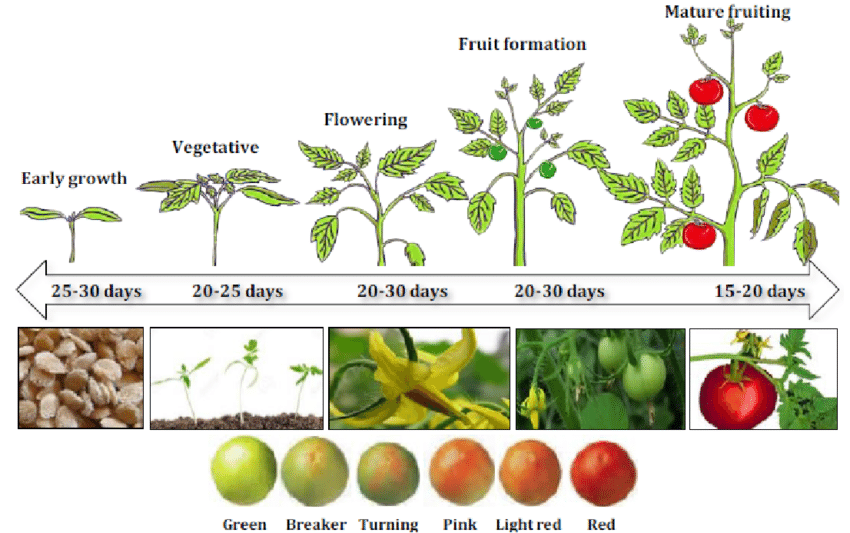
\includegraphics[width=1.0\textwidth]{user-view/growth_stages.png}
    \caption{\enquote{Demonstration of the five growth stages of tomato, and the different levels of fruit ripeness.} \cite{Shamshiri2018}}
    \label{growth-stages}
\end{figure}

In later growth stages, additional branch structures appear above pre-exiting branches creating a level-like
plants appearance whereby older branches are longer and newly grown branches are naturally shorter.\\

Tomato fruits are healthy and ripe once their surface is covered entirely in an rather dark red.
There also exist other varieties of tomatoes which yield to yellow or green ripe fruits but those
or not used here.

\subsubsection*{Leaves}

The main driver for bio-activity in plants is initiated through photosynthetic active radiation (PAR)
through the impact of light on the leaf surface and interaction with gas.
Depending on the growth stage and lighting conditions the leaf surface can appear differently.

In earlier growth stages the leaves are light green and slightly translucent (figure \ref{fig:trans}).
In later growing stages the leaf textures is typically a darker green, hairy and covered
with a wax making the leaves appear mostly mat and dark green (figure \ref{fig:wax}).

\begin{figure}[H]
    \centering
    \begin{minipage}[b]{0.49\textwidth}
        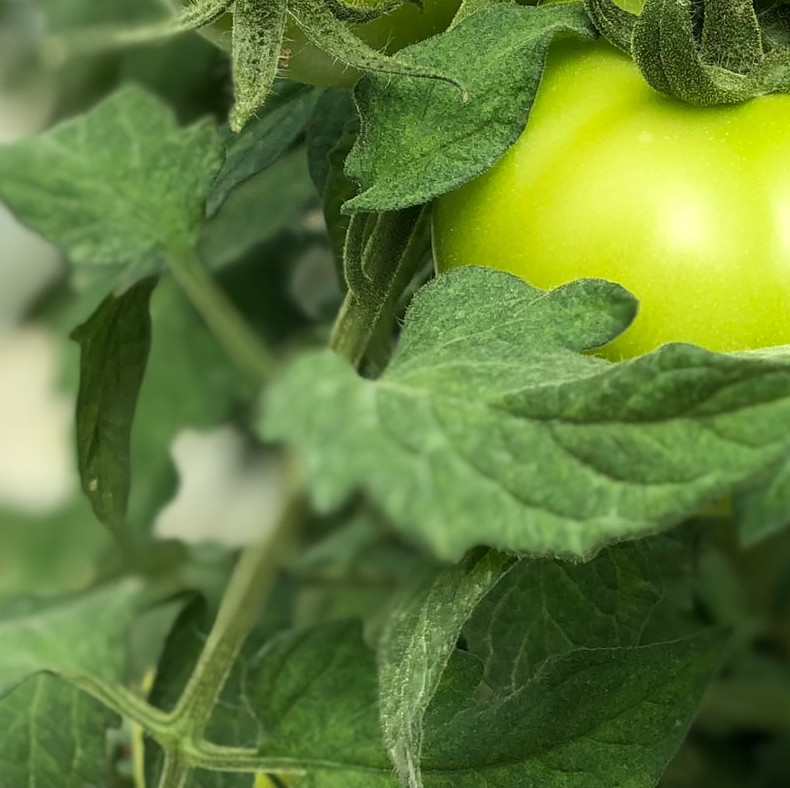
\includegraphics[width=\textwidth]{user-view/plant4_leaf_Soo_Ann_Woon_Unsplash.jpg}
        \caption{Hairy, waxy leaf surface}
        \label{fig:wax}
    \end{minipage}
    \hfill
    \begin{minipage}[b]{0.49\textwidth}
        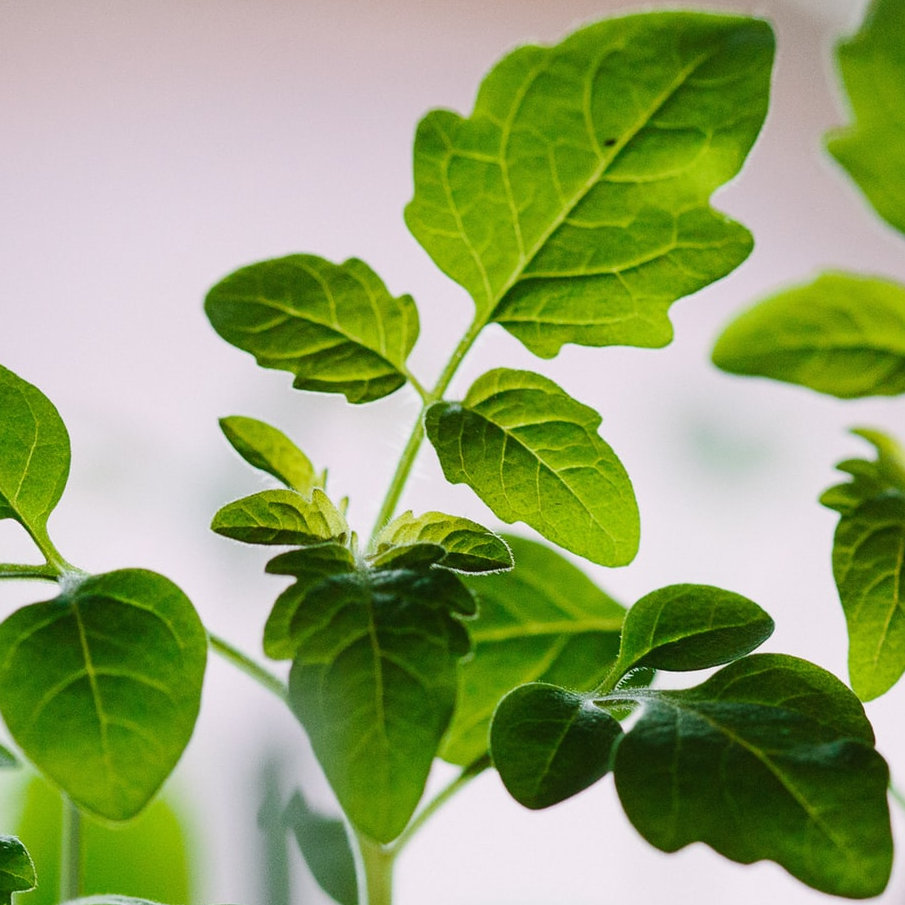
\includegraphics[width=\textwidth]{user-view/plant2_Francesco_Gallarotti_unsplash.jpg}
        \caption{Young leaves partly translucent}
        \label{fig:trans}
    \end{minipage}
\end{figure}

\subsubsection*{Defective Plants}

Defects in plants are either apparent through visibly damaged leaves, fruits or both.
Healthy leaves which contribute to the plant's bio-activity - and hence its yield - are throughout green
and do not contain other colors or physical damages.
Damaged fruits are also apparent through drastic color differences along the surface ,
like red-like and black or red and orange.

Figure \ref{fig:septoria} and \ref{fig:blight} show the two most common diseases which are visible through leave changes and
figure \ref{fig:Anthracnose} and \ref{fig:blossom} and show the two most common fruit diseases - both are caused by fungi
and lead to unusable yield \cite{diseases}.

\begin{figure}[H]
    \centering
    \begin{minipage}[b]{0.45\textwidth}
        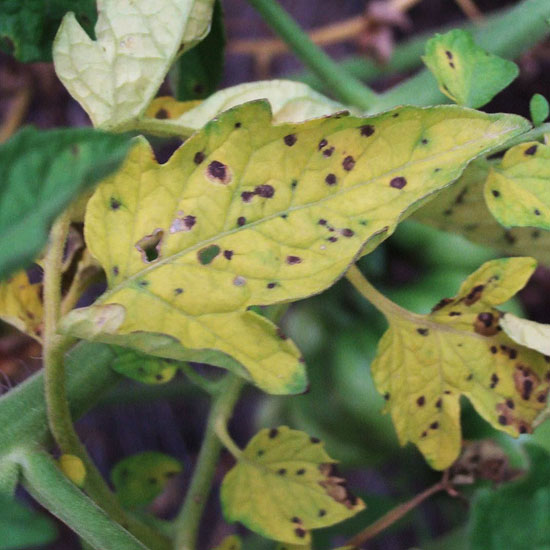
\includegraphics[width=\textwidth]{user-view/sick_0.jpg}
        \caption{Septoria Leaf Spot: Fungus}
        \label{fig:septoria}
    \end{minipage}
    \hfill
    \begin{minipage}[b]{0.45\textwidth}
        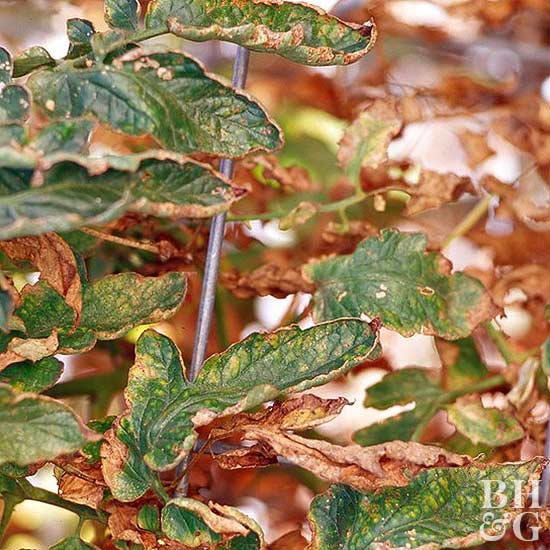
\includegraphics[width=\textwidth]{user-view/sick_1.jpg}
        \caption{Early Blight: Fungus}
        \label{fig:blight}
    \end{minipage}
\end{figure}

As visible the fungi affect leaf surface and color. Both have deviating color and texture
as expected from green healthy leaves.

\begin{figure}[H]
    \centering
    \begin{minipage}[b]{0.45\textwidth}
        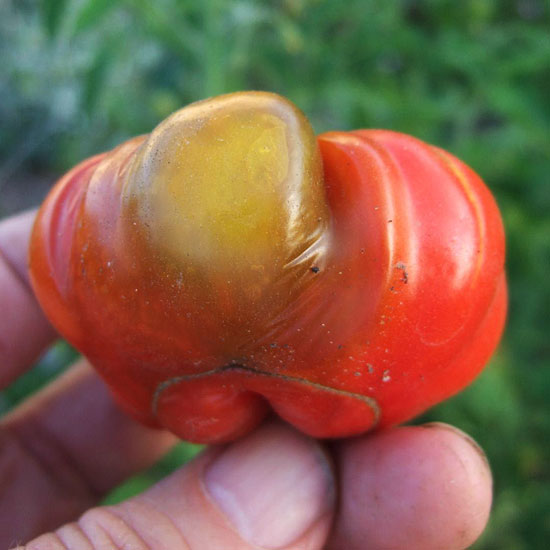
\includegraphics[width=\textwidth]{user-view/sick_2.jpg}
        \caption{Anthracnose: Fungus}
        \label{fig:Anthracnose}
    \end{minipage}
    \hfill
    \begin{minipage}[b]{0.45\textwidth}
        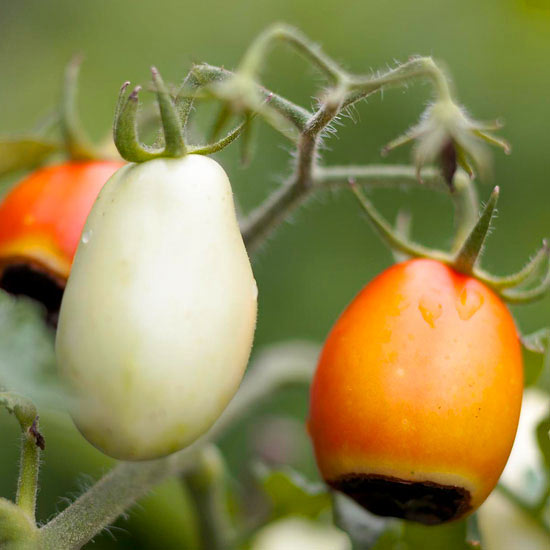
\includegraphics[width=\textwidth]{user-view/sick_3.jpg}
        \caption{Blossom-End Rot}
        \label{fig:blossom}
    \end{minipage}
\end{figure}

Damaged fruits are visible through big differently color clusters along the surface.

\clearpage
\subsection{Task Requirements}\label{subsec:task-requirements}

This project is concerned with the commercial domain of yield production and its purpose
is to predict yield, hence the goal is to design a solution which can automatically estimate yield:\\

For this purpose the requirements are:

\begin{enumerate}
    \item Estimate yield based on camera images taken from tomato plants within a greenhouse
    \item the greenhouse space should be used as effective as possible, means that the number of plants per group unit should be dense
    and ideally no rearrangement is necessary and mainly minimal additional equipment is needed
\end{enumerate}
\newpage
